\documentclass[journal, a4paper]{IEEEtran}

% some very useful LaTeX packages include:

%\usepackage{cite}      % Written by Donald Arseneau
                        % V1.6 and later of IEEEtran pre-defines the format
                        % of the cite.sty package \cite{} output to follow
                        % that of IEEE. Loading the cite package will
                        % result in citation numbers being automatically
                        % sorted and properly "ranged". i.e.,
                        % [1], [9], [2], [7], [5], [6]
                        % (without using cite.sty)
                        % will become:
                        % [1], [2], [5]--[7], [9] (using cite.sty)
                        % cite.sty's \cite will automatically add leading
                        % space, if needed. Use cite.sty's noadjust option
                        % (cite.sty V3.8 and later) if you want to turn this
                        % off. cite.sty is already installed on most LaTeX
                        % systems. The latest version can be obtained at:
                        % http://www.ctan.org/tex-archive/macros/latex/contrib/supported/cite/

\usepackage{graphicx}   % Written by David Carlisle and Sebastian Rahtz
                        % Required if you want graphics, photos, etc.
                        % graphicx.sty is already installed on most LaTeX
                        % systems. The latest version and documentation can
                        % be obtained at:
                        % http://www.ctan.org/tex-archive/macros/latex/required/graphics/
                        % Another good source of documentation is "Using
                        % Imported Graphics in LaTeX2e" by Keith Reckdahl
                        % which can be found as esplatex.ps and epslatex.pdf
                        % at: http://www.ctan.org/tex-archive/info/

%\usepackage{psfrag}    % Written by Craig Barratt, Michael C. Grant,
                        % and David Carlisle
                        % This package allows you to substitute LaTeX
                        % commands for text in imported EPS graphic files.
                        % In this way, LaTeX symbols can be placed into
                        % graphics that have been generated by other
                        % applications. You must use latex->dvips->ps2pdf
                        % workflow (not direct pdf output from pdflatex) if
                        % you wish to use this capability because it works
                        % via some PostScript tricks. Alternatively, the
                        % graphics could be processed as separate files via
                        % psfrag and dvips, then converted to PDF for
                        % inclusion in the main file which uses pdflatex.
                        % Docs are in "The PSfrag System" by Michael C. Grant
                        % and David Carlisle. There is also some information
                        % about using psfrag in "Using Imported Graphics in
                        % LaTeX2e" by Keith Reckdahl which documents the
                        % graphicx package (see above). The psfrag package
                        % and documentation can be obtained at:
                        % http://www.ctan.org/tex-archive/macros/latex/contrib/supported/psfrag/

%\usepackage{subfigure} % Written by Steven Douglas Cochran
                        % This package makes it easy to put subfigures
                        % in your figures. i.e., "figure 1a and 1b"
                        % Docs are in "Using Imported Graphics in LaTeX2e"
                        % by Keith Reckdahl which also documents the graphicx
                        % package (see above). subfigure.sty is already
                        % installed on most LaTeX systems. The latest version
                        % and documentation can be obtained at:
                        % http://www.ctan.org/tex-archive/macros/latex/contrib/supported/subfigure/

\usepackage{url}        % Written by Donald Arseneau
                        % Provides better support for handling and breaking
                        % URLs. url.sty is already installed on most LaTeX
                        % systems. The latest version can be obtained at:
                        % http://www.ctan.org/tex-archive/macros/latex/contrib/other/misc/
                        % Read the url.sty source comments for usage information.

%\usepackage{stfloats}  % Written by Sigitas Tolusis
                        % Gives LaTeX2e the ability to do double column
                        % floats at the bottom of the page as well as the top.
                        % (e.g., "\begin{figure*}[!b]" is not normally
                        % possible in LaTeX2e). This is an invasive package
                        % which rewrites many portions of the LaTeX2e output
                        % routines. It may not work with other packages that
                        % modify the LaTeX2e output routine and/or with other
                        % versions of LaTeX. The latest version and
                        % documentation can be obtained at:
                        % http://www.ctan.org/tex-archive/macros/latex/contrib/supported/sttools/
                        % Documentation is contained in the stfloats.sty
                        % comments as well as in the presfull.pdf file.
                        % Do not use the stfloats baselinefloat ability as
                        % IEEE does not allow \baselineskip to stretch.
                        % Authors submitting work to the IEEE should note
                        % that IEEE rarely uses double column equations and
                        % that authors should try to avoid such use.
                        % Do not be tempted to use the cuted.sty or
                        % midfloat.sty package (by the same author) as IEEE
                        % does not format its papers in such ways.

\usepackage{amsmath}    % From the American Mathematical Society
                        % A popular package that provides many helpful commands
                        % for dealing with mathematics. Note that the AMSmath
                        % package sets \interdisplaylinepenalty to 10000 thus
                        % preventing page breaks from occurring within multiline
                        % equations. Use:
%\interdisplaylinepenalty=2500
                        % after loading amsmath to restore such page breaks
                        % as IEEEtran.cls normally does. amsmath.sty is already
                        % installed on most LaTeX systems. The latest version
                        % and documentation can be obtained at:
                        % http://www.ctan.org/tex-archive/macros/latex/required/amslatex/math/



% Other popular packages for formatting tables and equations include:

%\usepackage{array}
% Frank Mittelbach's and David Carlisle's array.sty which improves the
% LaTeX2e array and tabular environments to provide better appearances and
% additional user controls. array.sty is already installed on most systems.
% The latest version and documentation can be obtained at:
% http://www.ctan.org/tex-archive/macros/latex/required/tools/

% V1.6 of IEEEtran contains the IEEEeqnarray family of commands that can
% be used to generate multiline equations as well as matrices, tables, etc.

% Also of notable interest:
% Scott Pakin's eqparbox package for creating (automatically sized) equal
% width boxes. Available:
% http://www.ctan.org/tex-archive/macros/latex/contrib/supported/eqparbox/

% *** Do not adjust lengths that control margins, column widths, etc. ***
% *** Do not use packages that alter fonts (such as pslatex).         ***
% There should be no need to do such things with IEEEtran.cls V1.6 and later.


% Your document starts here!
\begin{document}
\begin{titlepage}

\newcommand{\HRule}{\rule{\linewidth}{0.5mm}} % Defines a new command for the horizontal lines, change thickness here

\center % Center everything on the page
 %----------------------------------------------------------------------------------------
%	LOGO SECTION
%----------------------------------------------------------------------------------------

~\\[1cm]

\includegraphics{SCUT.png}\\[2cm] % Include a department/university logo - this will require the graphicx package

%----------------------------------------------------------------------------------------
%	TITLE SECTION
%----------------------------------------------------------------------------------------

\HRule \\[1cm]
{ \huge \bfseries The Experiment Report of \textit{Machine Learning} }\\[0.6cm] % Title of your document
\HRule \\[2cm]
%----------------------------------------------------------------------------------------
%	HEADING SECTIONS
%----------------------------------------------------------------------------------------


\textsc{\LARGE \textbf{School:} School of Software Engineering}\\[1cm]
\textsc{\LARGE \textbf{Subject:} Software Engineering}\\[2cm] 

 
%----------------------------------------------------------------------------------------
%	AUTHOR SECTION
%----------------------------------------------------------------------------------------

\begin{minipage}{0.4\textwidth}
\begin{flushleft} \large
\emph{Author:}\\
Biquan Wang % Your name
\end{flushleft}
\end{minipage}
~
\begin{minipage}{0.4\textwidth}
\begin{flushright} \large
\emph{Supervisor:} \\
Qingyao Wu % Supervisor's Name
\end{flushright}
\end{minipage}\\[2cm]
~
\begin{minipage}{0.4\textwidth}
\begin{flushleft} \large
\emph{Student ID:}\\
201821038853
\end{flushleft}
\end{minipage}
~
\begin{minipage}{0.4\textwidth}
\begin{flushright} \large
\emph{Grade:} \\
Graduate
\end{flushright}
\end{minipage}\\[2cm]

% If you don't want a supervisor, uncomment the two lines below and remove the section above
%\Large \emph{Author:}\\
%John \textsc{Smith}\\[3cm] % Your name

%----------------------------------------------------------------------------------------
%	DATE SECTION
%----------------------------------------------------------------------------------------

{\large \today}\\[2cm] % Date, change the \today to a set date if you want to be precise

 
%----------------------------------------------------------------------------------------

\vfill % Fill the rest of the page with whitespace

\end{titlepage}

% Define document title and author
	\title{Linear Regression and Stochastic Gradient Descent}
	\maketitle

% Write abstract here
\begin{abstract}
Linear regression is one of the simplest and most important model of machine learning. This report try two show the process of closed-form solution and gradient descent of linear regression. Futher more, we try to prove the validity of gradient descent and show the loss with different learning rate. 
\end{abstract}

% Each section begins with a \section{title} command
\section{Introduction}
	% \PARstart{}{} creates a tall first letter for this first paragraph
\PARstart{L}{inear} regression is a linear approach to modelling the relationship between a scalar response and one or more explanatory variables. It is one of the simplest and important model of machine learning. Stochastic gradient descent is one of the most popular algorithms of optimization and was often used as black-box optimizer. This method is widely used in neural networks.

This report aims to show the process of closed-form solution and stochastic gradient descent of linear regression. It also contains the result of closed-form solution, the compare between the loss of closed-fromr solution, full-batch gradient descent, and mini-batch stochastic gradient descent, which can prove the validity of MSGD and FGD. Futher more,  we provided the result of FGD and MSGD. 

% Main Part
\section{Methods and Theory}
In this section, we will give a complete introduction to the experiment, which contains the theory and function of closed-form solution, the losss function and stohcastic gradient descent of linear regression.

The regularized least square regression:
\begin{displaymath}
\boldsymbol{L}_D(\boldsymbol{w})=\frac{\lambda}{2}||\boldsymbol{w}||^{2}_2 + \frac{1}{2}\sum_{i=1}^n(y_i-f(\boldsymbol{x_i};\boldsymbol{w}))^2
\end{displaymath}
\begin{eqnarray}
\boldsymbol{L}_D(\boldsymbol{w})=\frac{\lambda}{2}||\boldsymbol{w}||^{2}_2 + \frac{1}{2}||\boldsymbol{y}-\boldsymbol{Xw}||_2^2
\end{eqnarray}
Here, $\frac{1}{2}||\boldsymbol{w}||_2^2$ is called Regularizer, $\lambda$ is called trade-off parameter or regularization parameter.
Find minimizer of least squared loss:
\begin{displaymath}
\boldsymbol{w}^*=arg\:min_{\boldsymbol{w}} \boldsymbol{L}_D(\boldsymbol{W})
\end{displaymath}
First-order condition of the optimal solution:
\begin{displaymath}
\frac{\partial\boldsymbol{L}(\boldsymbol{w})}{\partial\boldsymbol{w}}=0
\end{displaymath}
For the least regression problem, we have:
\begin{eqnarray}
\frac{\partial\boldsymbol{L}(\boldsymbol{w})}{\partial\boldsymbol{w}}=\lambda\boldsymbol{w}-\boldsymbol{X}^T\boldsymbol{y}+\boldsymbol{X}^T\boldsymbol{Xw}
\end{eqnarray}
\begin{displaymath}
\lambda\boldsymbol{w}-\boldsymbol{X}^T\boldsymbol{y}+\boldsymbol{X}^T\boldsymbol{Xw}=0
\end{displaymath}
\begin{displaymath}
(\lambda\boldsymbol{I}+\boldsymbol{X}^T\boldsymbol{X})\boldsymbol{w}=\boldsymbol{X}^T\boldsymbol{y}
\end{displaymath}
\begin{displaymath}
\boldsymbol{w}=(\boldsymbol{X}^T\boldsymbol{X}+\lambda\boldsymbol{I})^-1\boldsymbol{X}^T\boldsymbol{y}
\end{displaymath}
We get the \textbf{closed-form solution} of linear regression:
\begin{eqnarray}
\boldsymbol{w}^*=(\boldsymbol{X}^T\boldsymbol{X}+\lambda\boldsymbol{I})^-1\boldsymbol{X}^T\boldsymbol{y}
\end{eqnarray}
\textbf{Gradient descent:}
\begin{itemize}
\item[-] Identify a set of hupotheses $f(\boldsymbol{x};\boldsymbol{w})$
\item[-] Define a loss criterion $\boldsymbol{L}_D$
\item[-] Pick the best $\boldsymbol{w}^*$ by minimizing a loss function $\boldsymbol{L}_D(\boldsymbol{w})$
\end{itemize}
\begin{displaymath}
arg\:min_{\boldsymbol{w}} \boldsymbol{L}_D(\boldsymbol{W})
\end{displaymath}
By Taylor expansion, when $\eta\to0$:
\begin{displaymath}
\boldsymbol{L}_D(\boldsymbol{w}+\eta\boldsymbol{d})=\boldsymbol{L}_D(\boldsymbol{w})+[\frac{\partial\boldsymbol{L}_D(\boldsymbol{w})}{\partial\boldsymbol{w}}]^T\eta\boldsymbol{d}+o(\eta\boldsymbol{d})
\end{displaymath}
\begin{displaymath}
\boldsymbol{L}_D(\boldsymbol{w}+\eta\boldsymbol{d})=\boldsymbol{L}_D(\boldsymbol{w})+\eta[\frac{\partial\boldsymbol{L}_D(\boldsymbol{w})}{\partial\boldsymbol{w}}]^T\boldsymbol{d}
\end{displaymath}
We have:
\begin{eqnarray}
\boldsymbol{L}_D(\boldsymbol{w'})=\boldsymbol{L}_D(\boldsymbol{w}+\eta\boldsymbol{d})\le\boldsymbol{L}_D(\boldsymbol{w})\quad(\eta\ne 0 \:\&\: \eta > 0)
\end{eqnarray}
We use $d=-\frac{\partial\boldsymbol{L}_D(\boldsymbol{w})}{\partial\boldsymbol{w}}$ as the direction of optimization.
Update parameters with rate $\eta$:
\begin{eqnarray}
\boldsymbol{w'}\rightarrow\boldsymbol{w}-\eta\frac{\partial\boldsymbol{L}_D(\boldsymbol{w})}{\partial\boldsymbol{w}}
\end{eqnarray}

In this experiment, we used \textbf{Mini-batch Stochastic Gradient Descent}, which means pick a part of data from train set randomly, and use this part of data to calculate the gradient and update the parameters. 

\section{Experiments}
This part contains two experiments, the first one is closed-form solution of linear regression, and the second part is linear regression with gradient descent. 
\subsection{Dataset}
Experiment uses the scaled edition of Housing in LIBSVM Data, including 506 samples and each sample has 13 features. 

\subsection{Experiment steps}
 \textbf{The steps of closed-form solution are as the following:}
\begin{itemize}
\item[1.] Use load\_svmlight\_file function in sklearn library to load the Housing scaled data.
\item[2.] Divide dataset into training set and validation set using train\_test\_split function.In these experiments, we set the validation size as 0.25.
\item[3.] Use closed-form solution (function (3)) to calculate the parameters $\boldsymbol{w}$ directly.
\item[4.] Use loss function (fucntion (1)) to calculate the loss on train set and validation set.
\end{itemize}

 \textbf{The steps of gradient descent solution are as the following:}
\begin{itemize}
\item[1.] Use load\_svmlight\_file function in sklearn library to load the Housing scaled data.
\item[2.] Divide dataset into training set and validation set using train\_test\_split function.In these experiments, we set the validation size as 0.25.
\item[3.]Initialize linear model parameters. Set all parameter into zero, initialize it randomly or with normal distribution.
\item[4.] Get a mini-batch data from train set randomly.
\item[5.] Update the parameters $\boldsymbol{w}$ with function (5)
\item[6.] Calculate the loss of train set and validation set with function (1).
\item[7.] Repeate setp 4-6 for n times, and return the losses of train set and validation set.

\subsection{Experiment result}
\begin{table}[!htb]
	\begin{center}
	\caption{Closed-form solution result}
	\label{tab:closed form}
	\begin{tabular}{|c|c|c|}
		\hline
		Type &  Loss of train set & Loss of valid set\\
		\hline
		Closed-form & 3.648082165263596 &3.5673788625276366 \\
		\hline
		FGD epoch200 & 3.5083401597660315 &4.233630428514219 \\
		\hline
		MSGD epoch200 & 3.777113540188303 &4.439968690213303 \\
		\hline
FGD epoch2000 & 3.449777991591353 &3.651855651969987 \\
		\hline
		MSGD epoch2000 & 3.454142930228637 & 3.653706861808154 \\
		\hline
	\end{tabular}
	\end{center}
\end{table}

Table.1 shows the result of closed-form solution, and compare with the loss of FGD and the loss of MSGD . We can find out from the table, with integration number increase, the difference of the loss of valid set and train set decreased, and both of them approch to closed-form loss.

The next part show the result of the experiment we have done for linear regression with gradient descent. All the figures, use plenty=0.5, epoch=200,batch size=200.

\end{itemize}
\begin{figure}[!htb]
	\begin{center}
	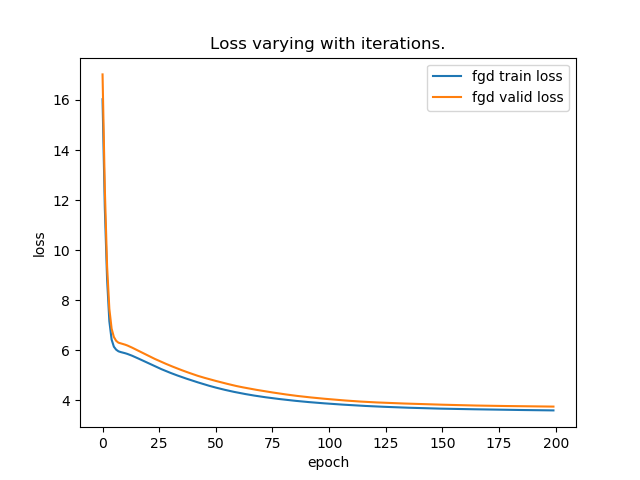
\includegraphics[width=\columnwidth]{lr_fgd}
	\caption{Full batch gradient descent of linear regression}
	\label{fig:lr_fgd}
	\end{center}
\end{figure}
\begin{figure}[!htb]
	\begin{center}
	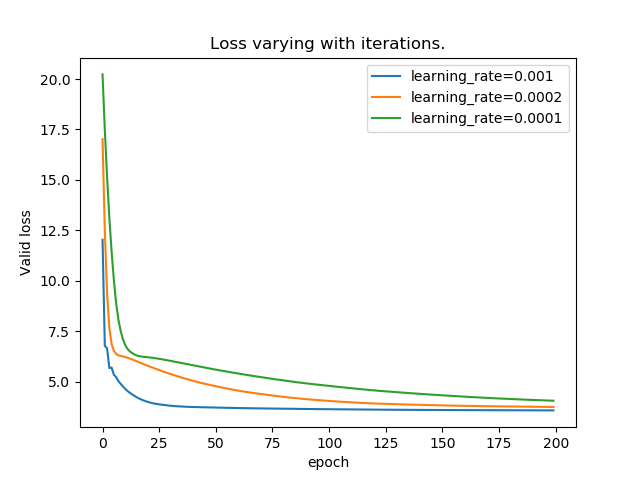
\includegraphics[width=\columnwidth]{lr_fgd_lr}
	\caption{Full batch gradient descent of linear regression}
	\label{fig:lr_fgd}
	\end{center}
\end{figure}
\begin{figure}[!htb]
	\begin{center}
	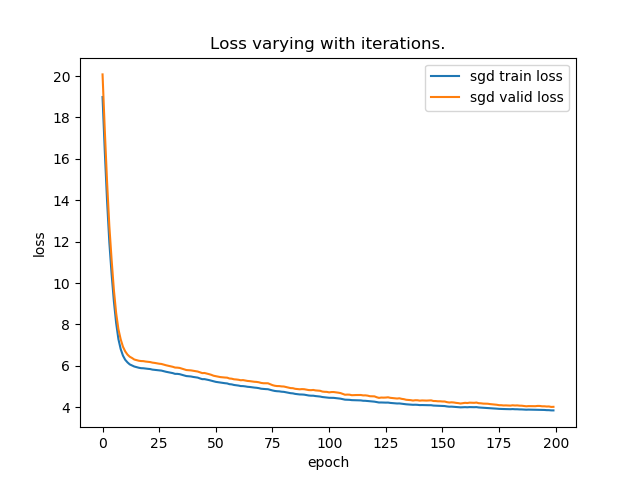
\includegraphics[width=\columnwidth]{lr_sgd}
	\caption{Mini-batch stochastic gradient descent of linear regression}
	\label{fig:lr_sgd}
	\end{center}
\end{figure}
\begin{figure}[!htb]
	\begin{center}
	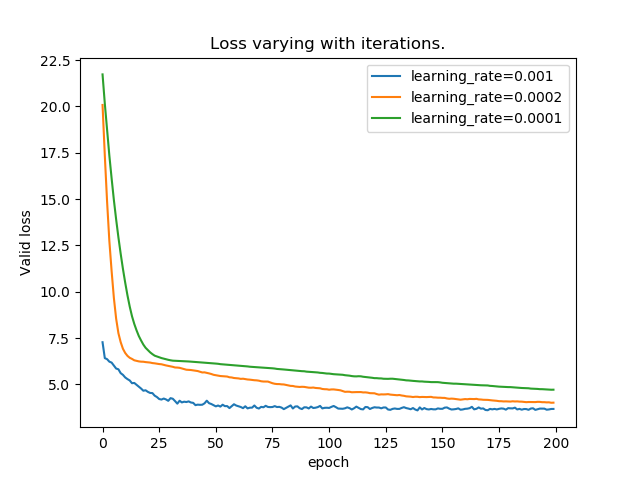
\includegraphics[width=\columnwidth]{lr_sgd_lr}
	\caption{Different learning rate MSGD of linear regression}
	\label{fig:lr_sgd_lr}
	\end{center}
\end{figure}

Fig.1 shows the result of Full batch gradient descent with learning rate 0.001.

Fig.2 compares different result of different learning rate of full match gradient descent. We can find out the loss descent more quick with the learn rate get bigger.

Fig.3 shows the valid loss and train loss of Mini-batch stochastic gradient descent with learning rate 0.0002.

Fig4. compares the result of Mini-batch stochastic gradient descent with different learning rate. When learn\_rate=0.001, the loss descent quickly and  starting to shake after 25 epoch.

\section{Conclusion}
	In this report, we mentioned two method of linear regression, Closed-form solution and Gradient descent. Closed-form solution can get the parameter $\boldsymbol{w}$ directly, but with the data set increase, this this method can not be relize. Mini-batch stochastic gradient descent is a solution of this situation, Table.1 shows this method can approch the result with the number of iterations increases.
\end{document}